\section{Цель работы}
Освоение принципов построения систем адаптивного управления на примере задачи слежения выхода скалярного объекта за эталонным сигналом.


\section{Теоретические сведения}
Рассматриваемый объект управления:
\begin{equation}
    \dot{x} = \theta x + u,
\end{equation}
где $x$~--- переменная состояния объекта, $u$~--- сигнал управления, $\theta$~--- неизвестный постоянный параметр.

Цель управления заключается в компенсации неопределенности $\theta$ и обеспечении следующего целевого равенства:
\begin{equation}\label{eq_goal_of_control}
    \lim_{t \rightarrow \infty} \bigl( x_m(t) - x(t) \bigr) = \lim_{t \rightarrow \infty} \varepsilon(t) = 0,
\end{equation}
где $\varepsilon = x_m - x$~--- ошибка управления, $x_m$~--- эталонный сигнал, являющийся выходом динамической модели вида (т.н. эталонной модели)
\begin{equation}
    \dot{x}_m = \lambda x_m + \lambda g,
\end{equation}
где $g$~--- сигнал задания, $\lambda$~--- параметр, задающий желаемое время переходного процесса.

Решающие поставленную задачу настраиваемый регулятор
\begin{equation}\label{eq_tuned_controller}
    u = -\hat{\theta} x - \lambda x + \lambda g
\end{equation}
и алгоритм адаптации
\begin{equation}\label{eq_AA}
    \dot{\hat{\theta}} = -\gamma x \varepsilon \ldotp
\end{equation}


\section{Исходные данные}
Варианту \textnumero2 соответствует следующий набор исходных данных:
\begin{equation}
    \theta = 2,
    \qquad
    \lambda = 2,
    \qquad
    g(t) = \cos 4t \ldotp
\end{equation}


\section{Результаты экспериментов}
См.~рисунки~\ref{img_first}--\ref{img_last} и подписи к ним.

\begin{figure}[h!]
    \centering
    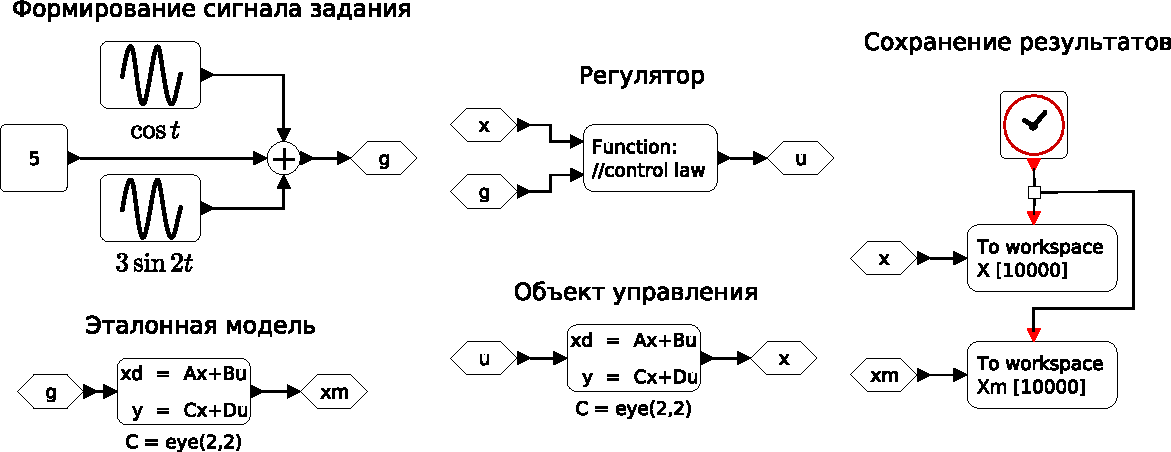
\includegraphics[width=\textwidth]{no_adapt.pdf}
    \caption{Схема моделирования процесса управления с помощью ненастраиваемого регулятора.}
    \label{img_first}
\end{figure}

\begin{figure}[h!]
    \centering
    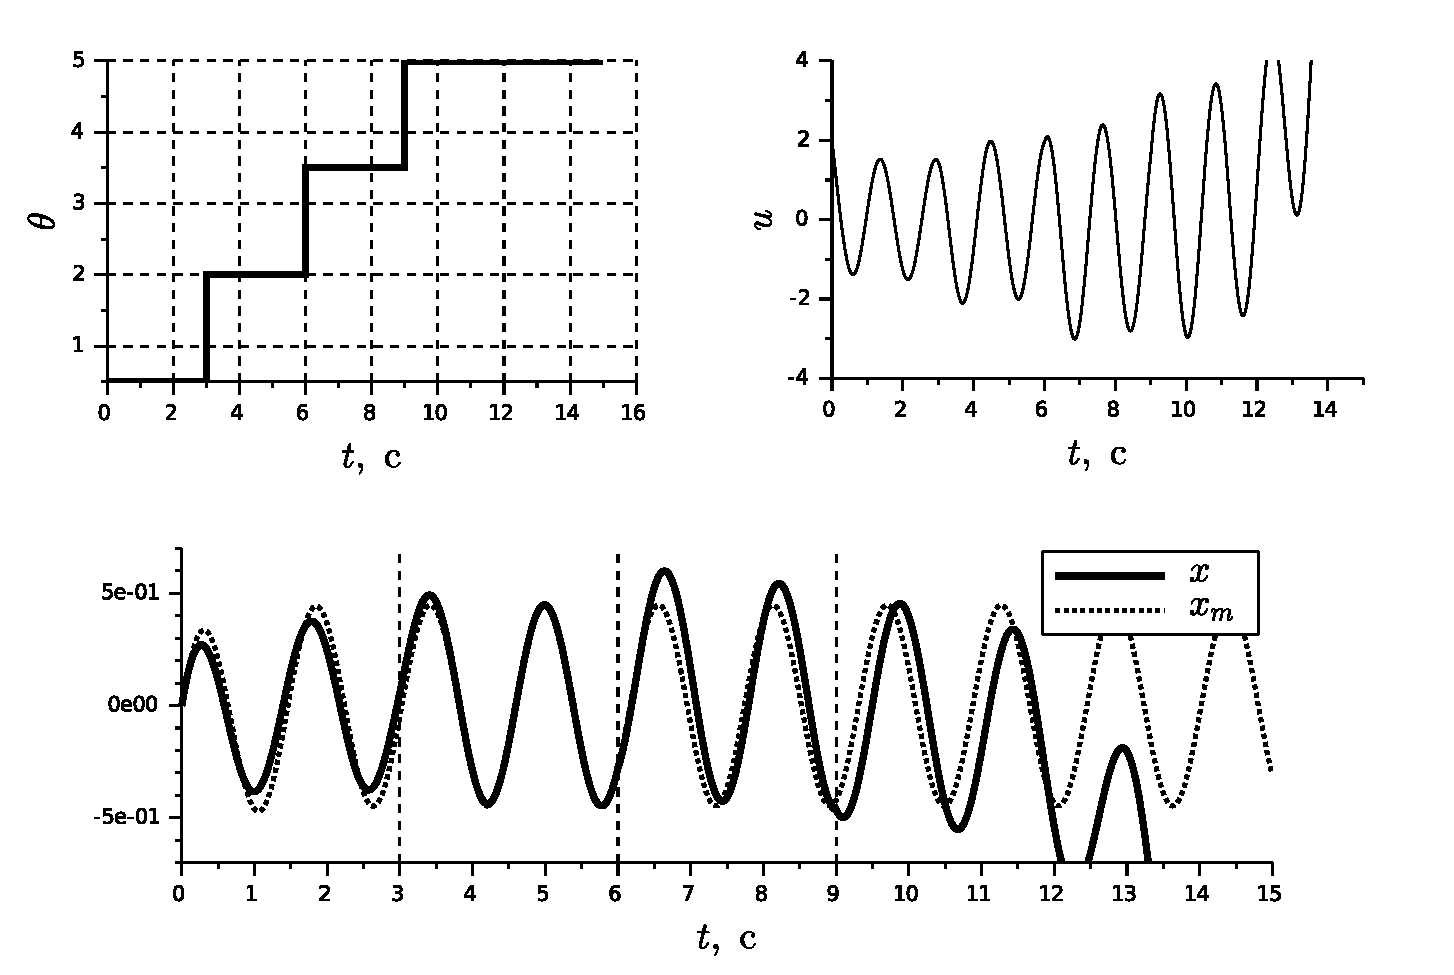
\includegraphics[width=\textwidth]{no_graphs.pdf}
    \caption{Результаты моделирования процесса управления с помощью ненастраиваемого регулятора.}
    \label{img_no_adapt_graphs}
\end{figure}

\begin{figure}[h!]
    \centering
    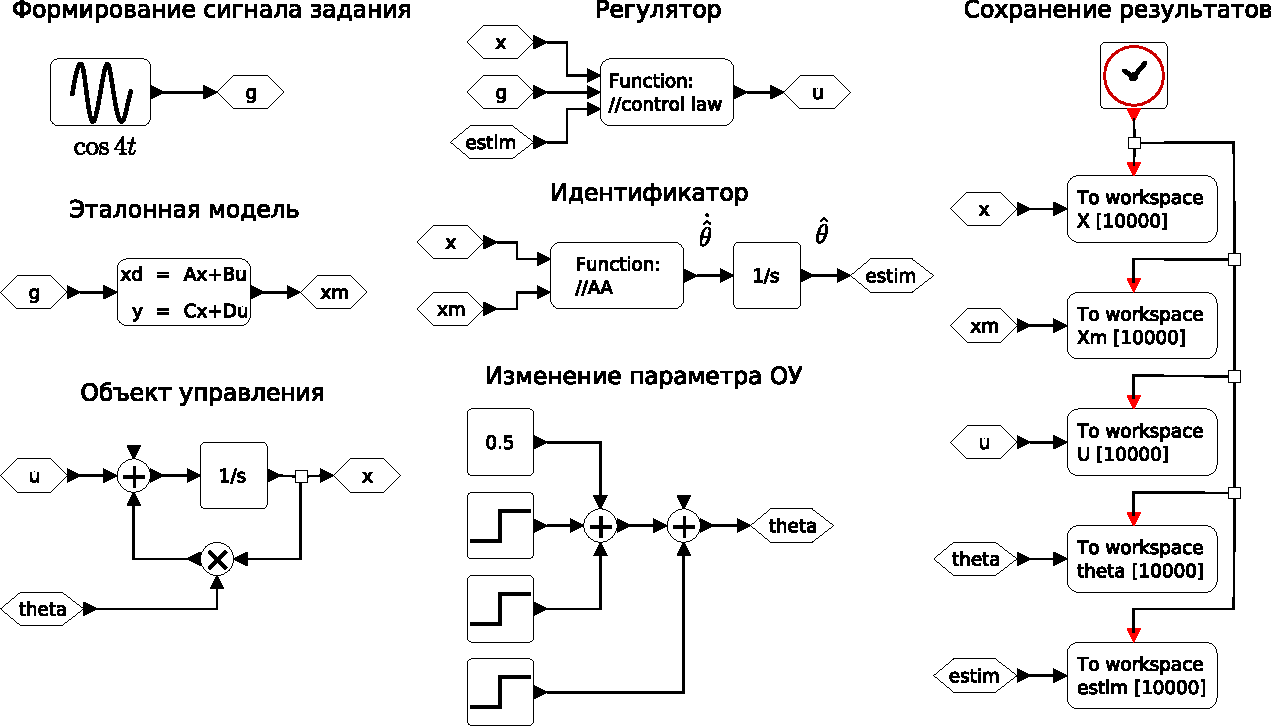
\includegraphics[width=\textwidth]{adapt.pdf}
    \caption{Схема моделирования процесса управления с помощью настраиваемого регулятора.}
\end{figure}

\begin{figure}[h!]
    \centering
    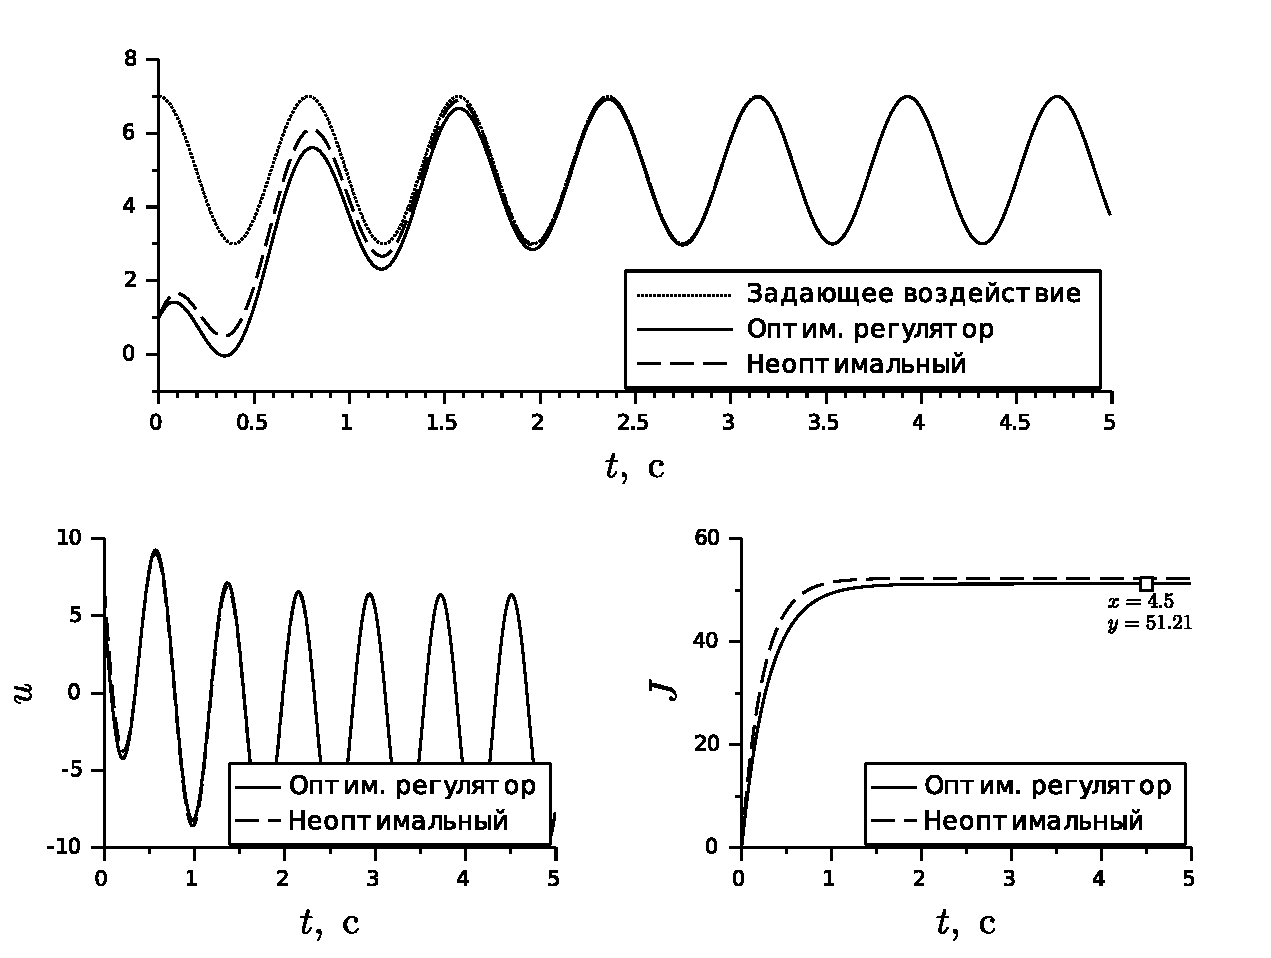
\includegraphics[width=\textwidth]{graphs.pdf}
    \caption{Результаты моделирования процесса управления с помощью настраиваемого регулятора при $\gamma=100$.}
    \label{img_adapt_graphs}
\end{figure}

\begin{figure}[h!]
    \centering
    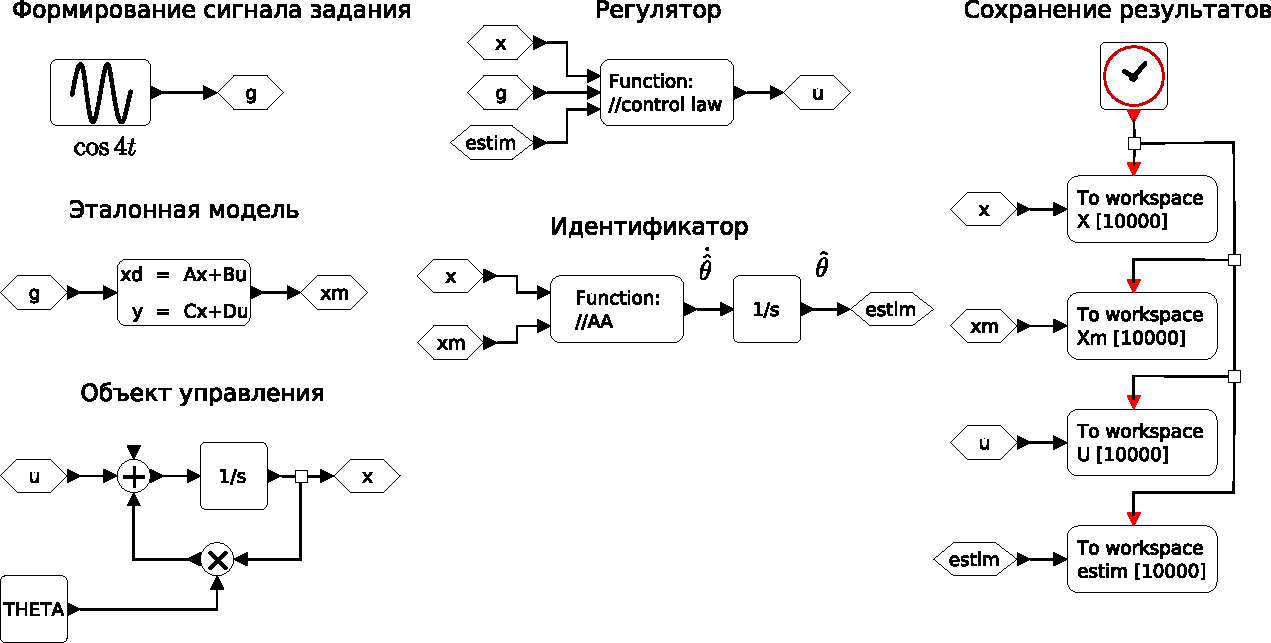
\includegraphics[width=\textwidth]{adapt_for_gamma_check.pdf}
    \caption{Схема моделирования, которая использовалась в экспериментах по выяснению влияния величины $\gamma$ на переходные процессы (\textsf{THETA=2}).}
\end{figure}

\begin{figure}[h!]
    \centering
    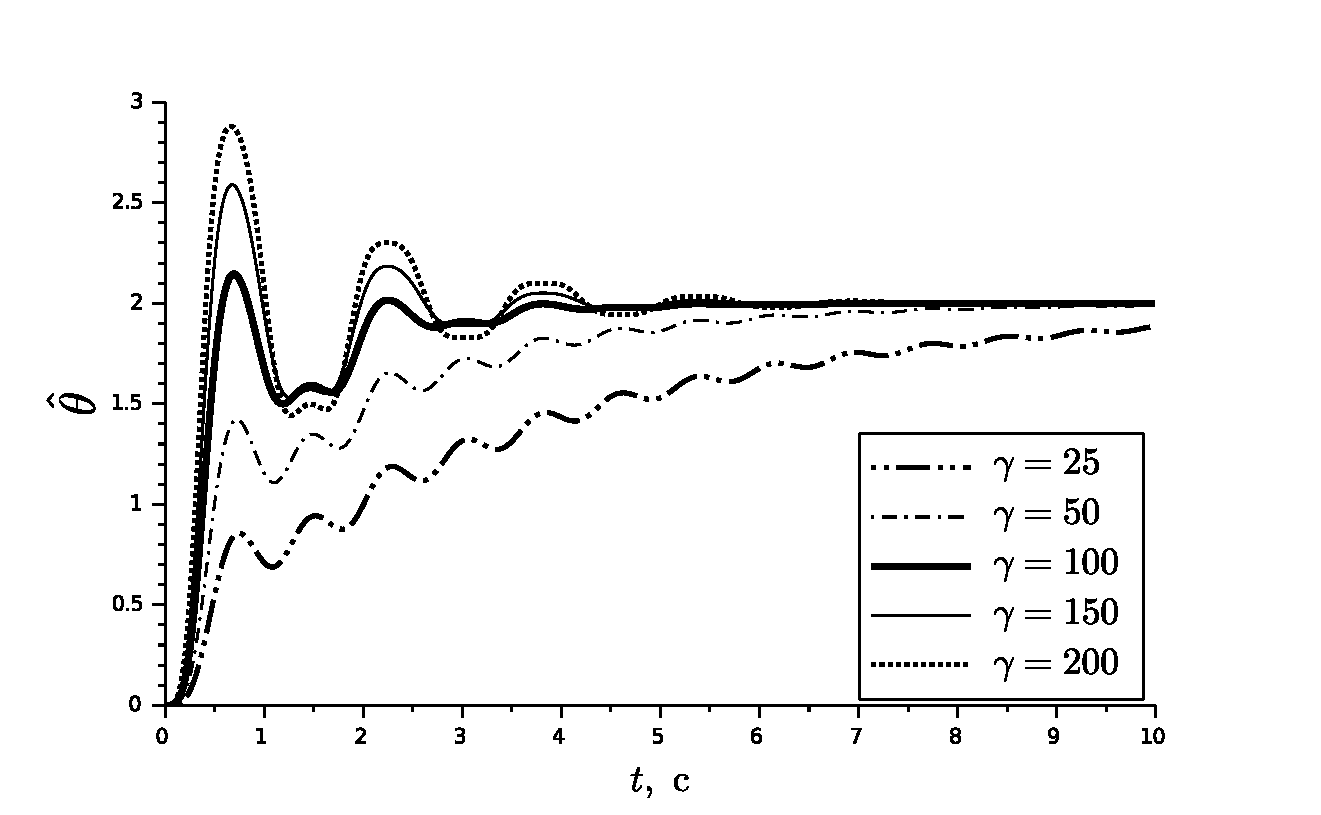
\includegraphics[width=0.9\textwidth]{diff_gammas_estims.pdf}
    \caption{Графики выходной величины идентификатора при разных значениях коэффициента адаптации.}
    \label{img_diff_gammas_estims}
\end{figure}

\begin{figure}[h!]
    \centering
    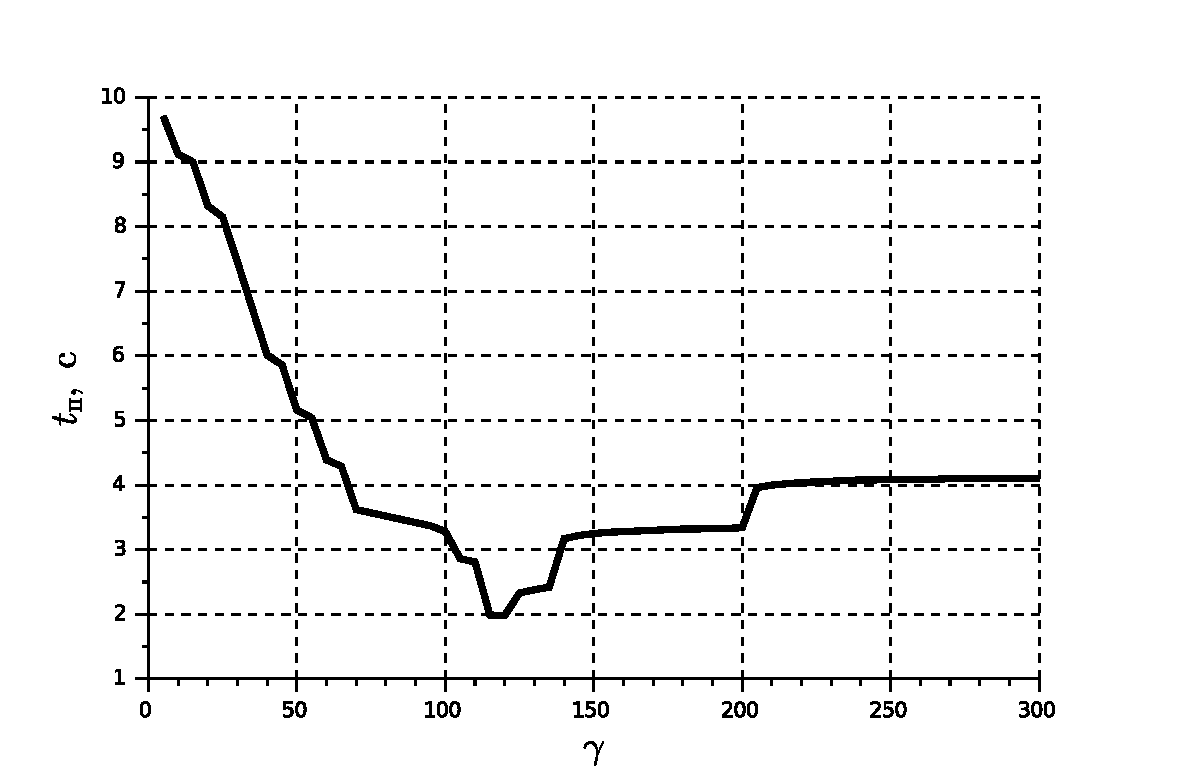
\includegraphics[width=0.75\textwidth]{time_of_gamma.pdf}
    \caption{График отражающий экспериментальную зависимость между временем переходного процесса кривой $\hat\theta(t)$ и значением коэффициента адаптации.}
    \label{img_time_of_gamma}
\end{figure}

\begin{figure}[h!]
    \centering
    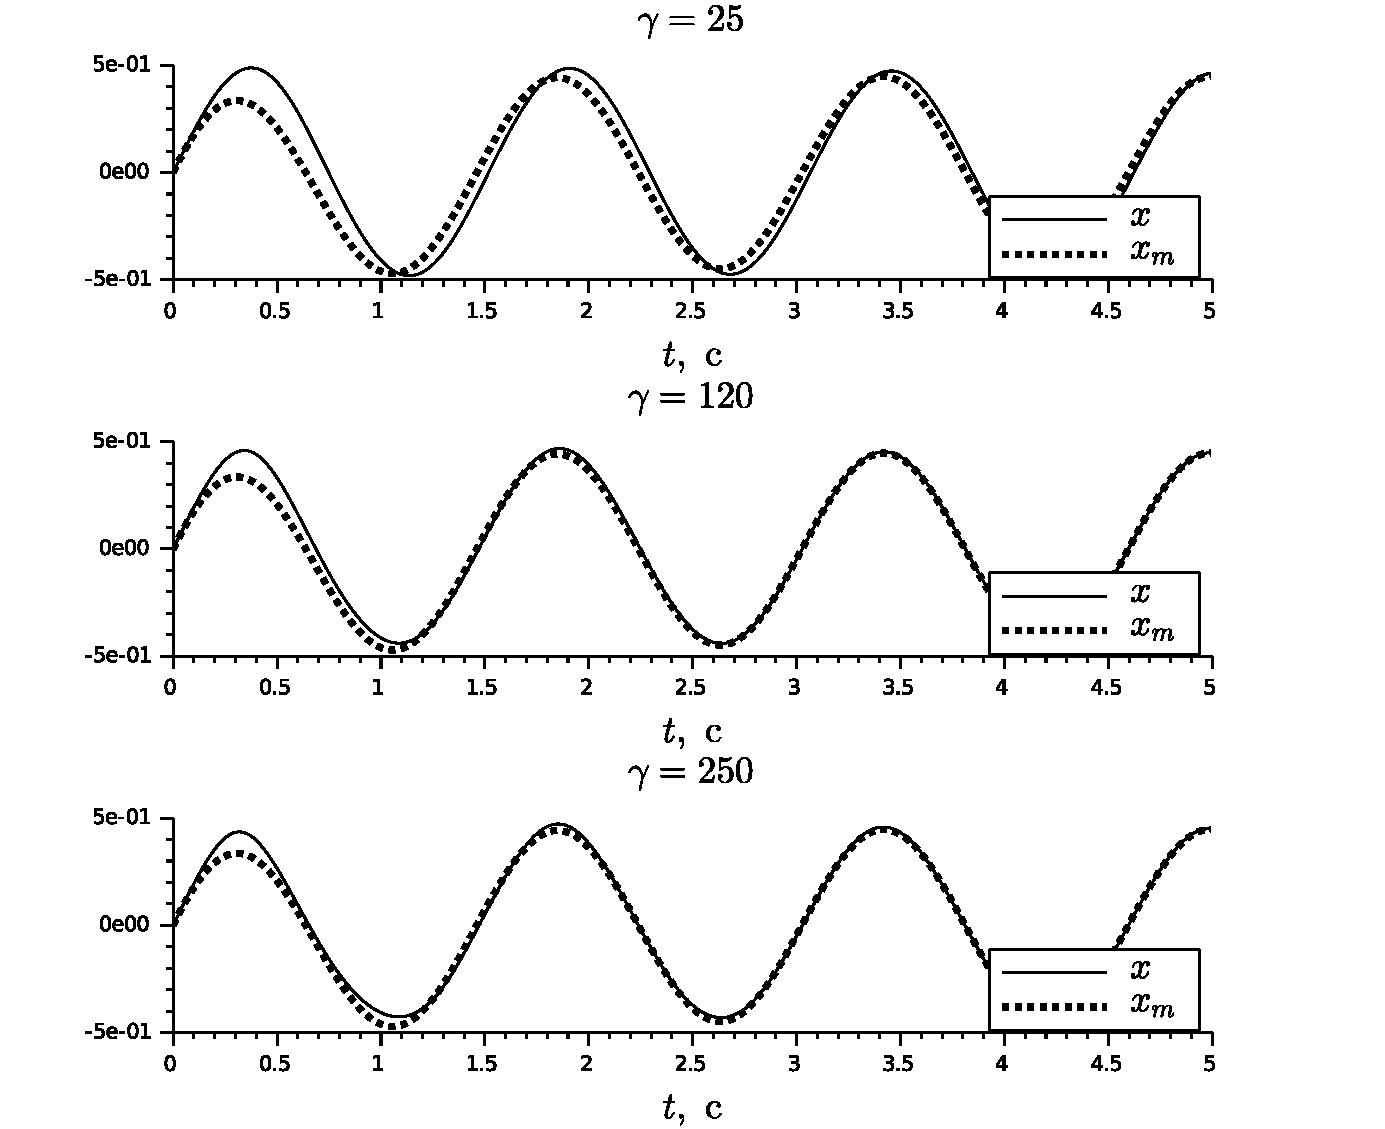
\includegraphics[width=0.89\textwidth]{diff_gammas_xs.pdf}
    \caption{Графики переходных процессов по состоянию объекта при разных значениях коэффициента адаптации.}
    \label{img_last}
\end{figure}

\newpage
\mbox{}
\newpage


\section{Выводы по работе}
В~результате проделанной работы экспериментальным путем было установлено, что
\begin{itemize}
    \item ненастраиваемый регулятор (получается из~\eqref{eq_tuned_controller} заменой $\hat{\theta}$ на $\theta$) в случае несовпадения значения $\theta$, используемого им для формирования управляющего воздействия~$u$, со значением одноименного параметра ОУ не только не выполняет целевого равенства~\eqref{eq_goal_of_control}, но и может не обеспечивать даже устойчивость ОУ (см.~рисунок~\ref{img_no_adapt_graphs});
    \item настраиваемый регулятор~\eqref{eq_tuned_controller} вкупе с алгоритмом адаптации~\eqref{eq_AA} решает поставленные задачи, заключающиеся в выполнении целевого условия~\eqref{eq_goal_of_control} и оценке значения неизвестного параметра $\theta$ объекта (см.~рисунок~\ref{img_adapt_graphs});
    \item значение коэффициента адаптации влияет на скорость (время) сходимости оценки $\hat{\theta}$ к истинному значению параметра $\theta$ ОУ (см.~рисунок~\ref{img_diff_gammas_estims}), при этом указанная зависимость имеет характер, иллюстрируемый графиком с рисунка~\ref{img_time_of_gamma}.
\end{itemize}